\section{Evaluation}\label{sec:evaluation}






\begin{figure}
  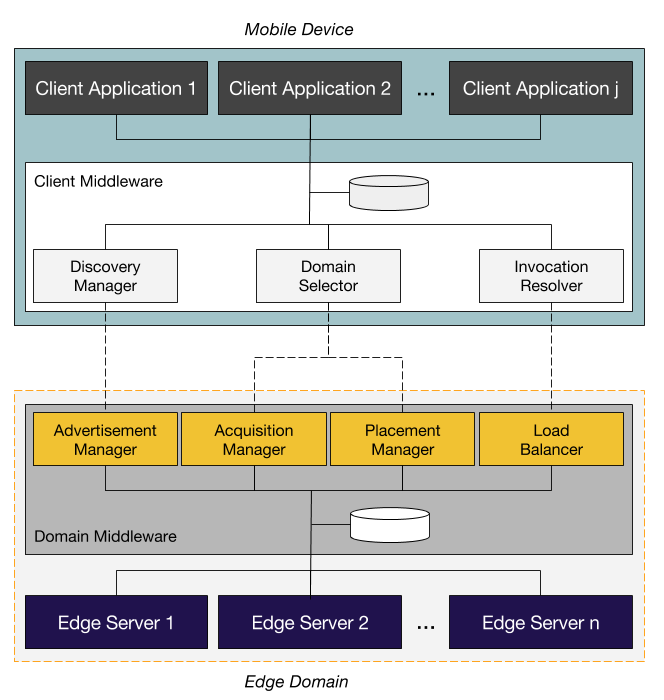
\includegraphics[width=0.6\textwidth]{figs/reference-architecture.png}
  \caption{TODO}
  \label{fig:reference-architecture}
\end{figure}

\begin{figure}
	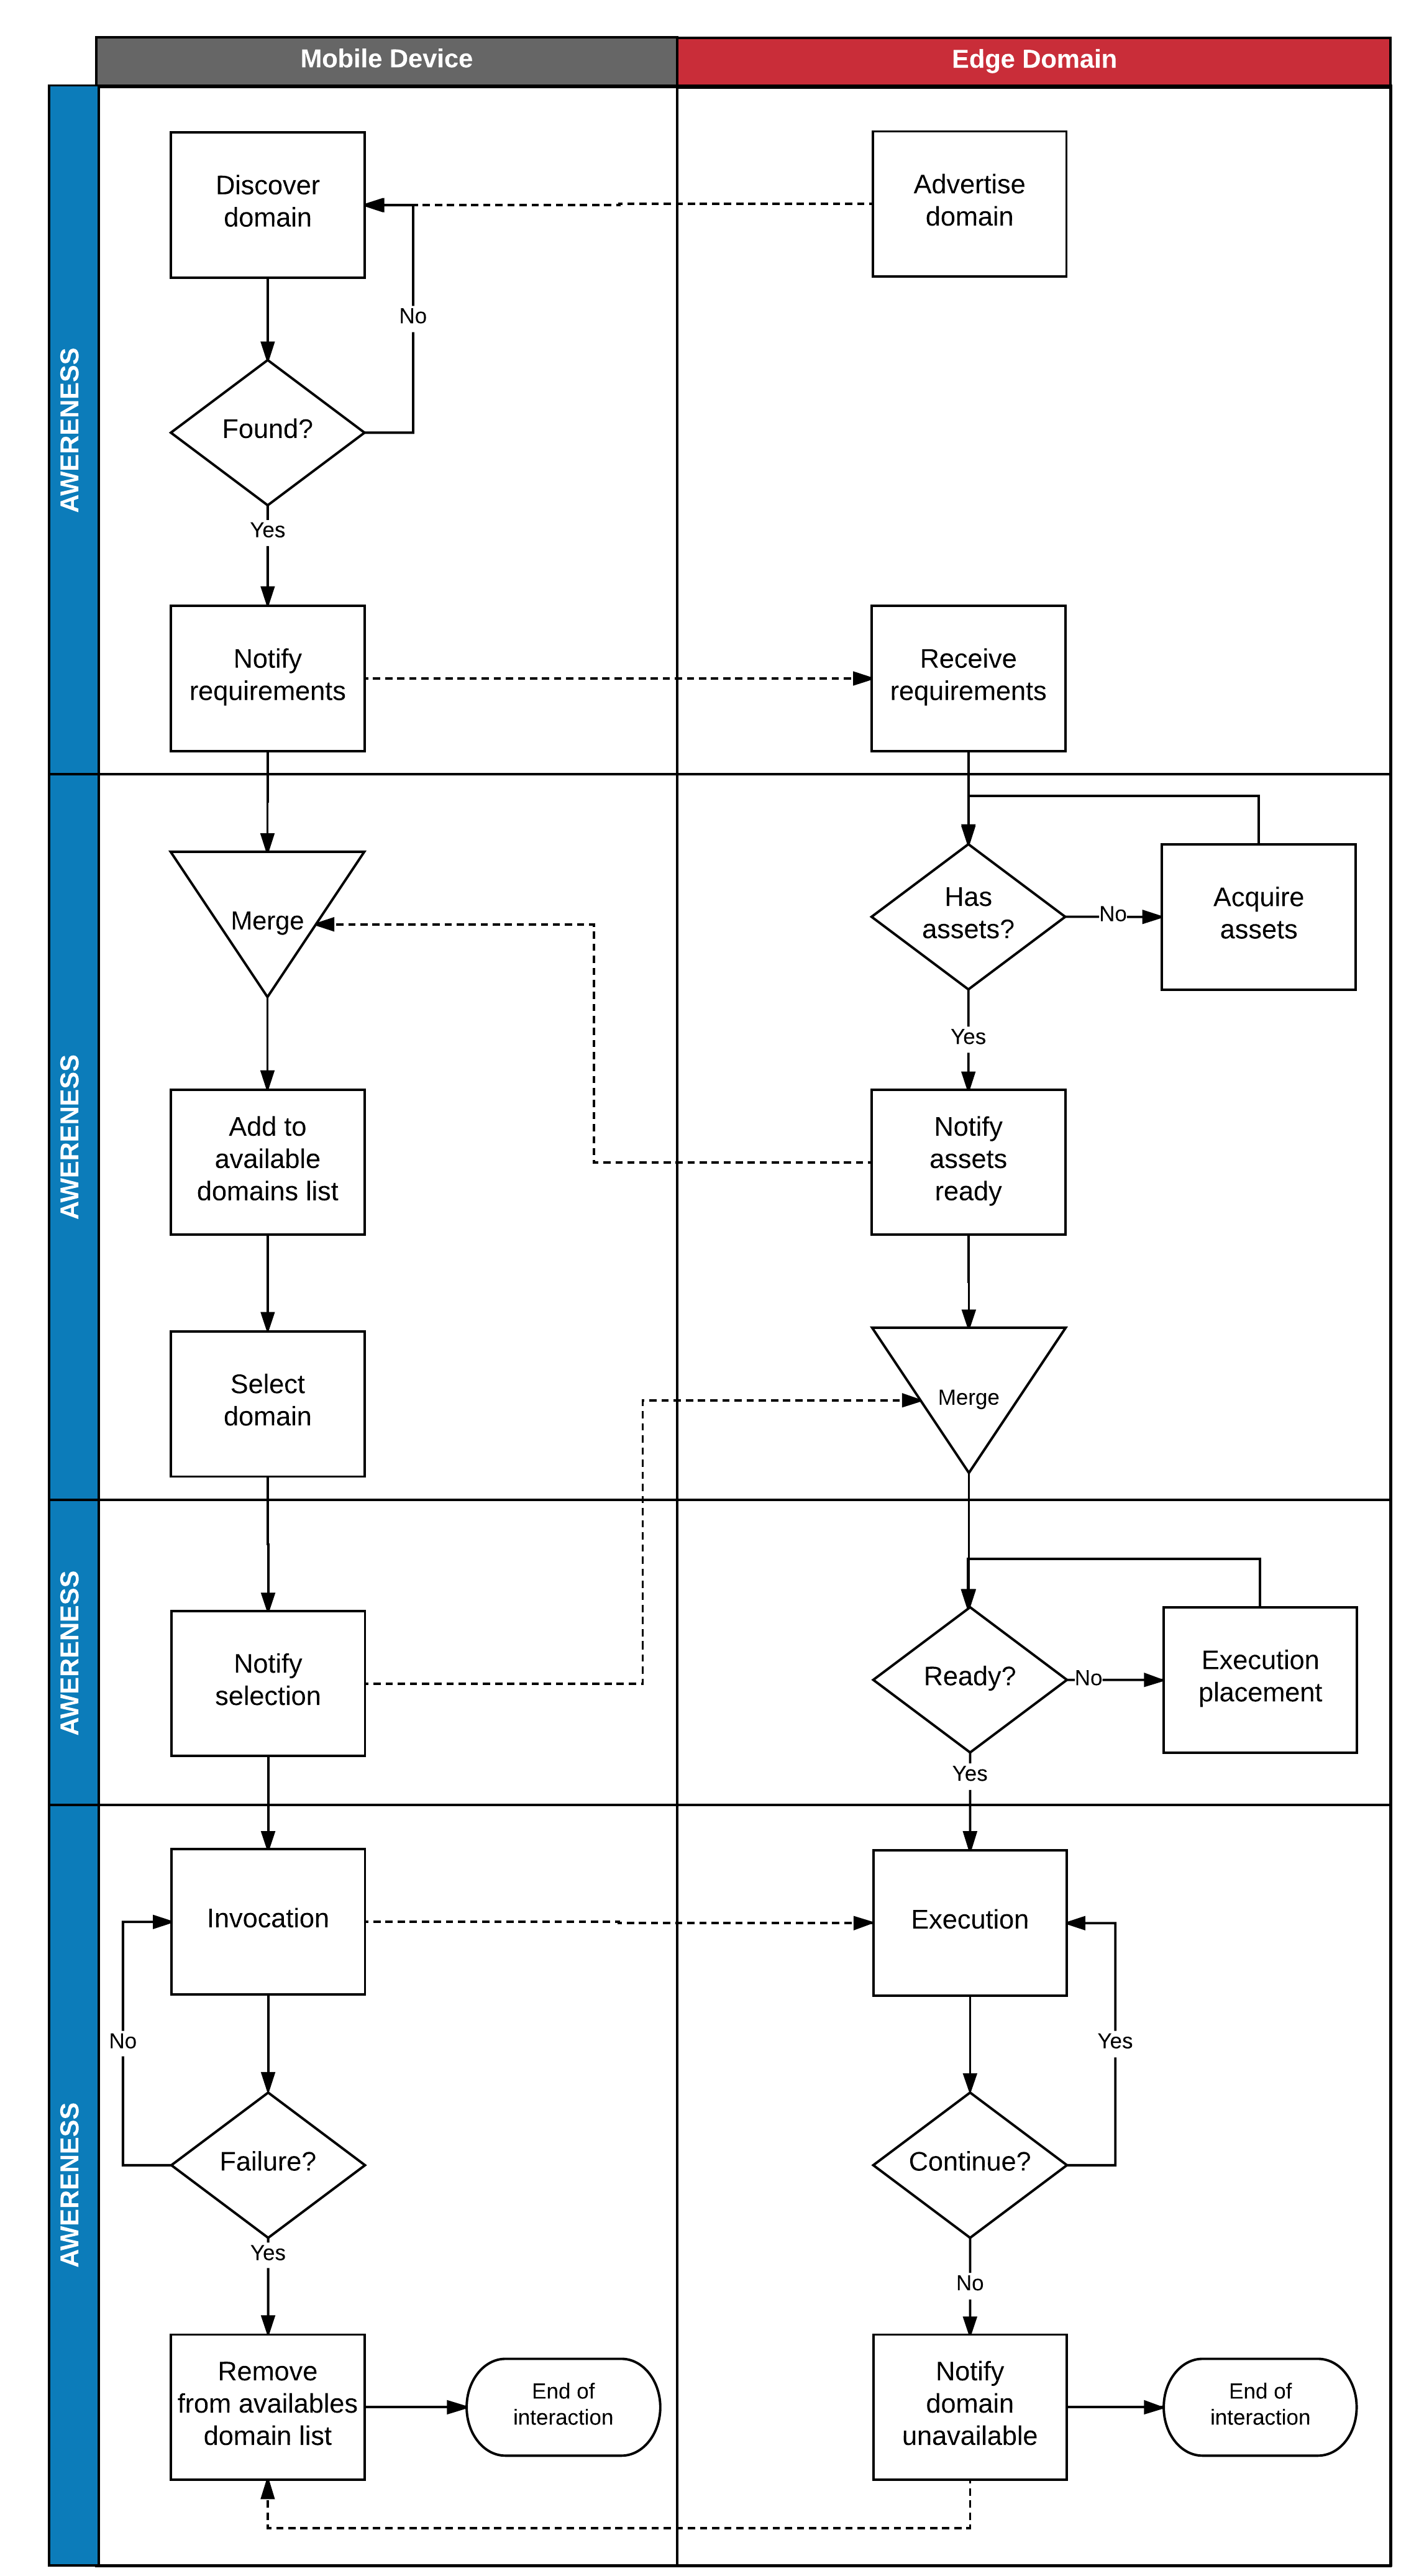
\includegraphics[height=\textheight]{figs/activities.png}
	\caption{TODO}
	\label{fig:activities}
\end{figure}

TODO: decide whether to leave activity diagram and details about HOW to perform each of the A3-E phases as part of the proposal or the evaluation; 

In accordance with requirement R1, edge domains perform the advertisement of their existence to whatever clients may be in reach. Potential clients, in their turn, must perform the discovery of edge domains. Before a given domain is found, it remains unknown to that client.

To address requirement R3 and R4, edge domains must remain free with respect to some application until the contact with a potential mobile client hosting that application. This condition refers to both the storage of application assets (e.g., code, libraries, etc), as well as the allocation of these assets for execution (e.g., deployment and instantiation of a restful application). 

Once a given domain has been discovered, the client must proceed with the identification of the application it is running. This process enables the edge domain to download whatever assets required by that specific application.  

The acquisition of application components does not make them ready to be executed. Instead, valuable resources like memory and CPU are kept free w.r.t. this application until the domain proceed with the placement of the application components as part of the allocation phase. The later activity corresponds to the allocation of resources from one or more domain servers required for the application execution. 	

Finally, once the allocation phase is finished, the domain is ready to perform the computation required by the application. For instance, following a request-response protocol, clients can fire requisitions to that domain. These activities are part of the engagement phase.

The separation of phases emphasizes not only the different concerns involved, but also the distinction between the moments they occur. The transition among phases may either be sequential, meaning that one phase starts as soon the previous finishes, or conditional, meaning that additional condition(s) must be met before the next phase can start. 	

%the client applications hosted by a mobile devices interact with a domain through a client middleware; the domain has its own middleware responsible for the activities in the A3-E model and interfaces with the servers in that domain


\begin{figure}
  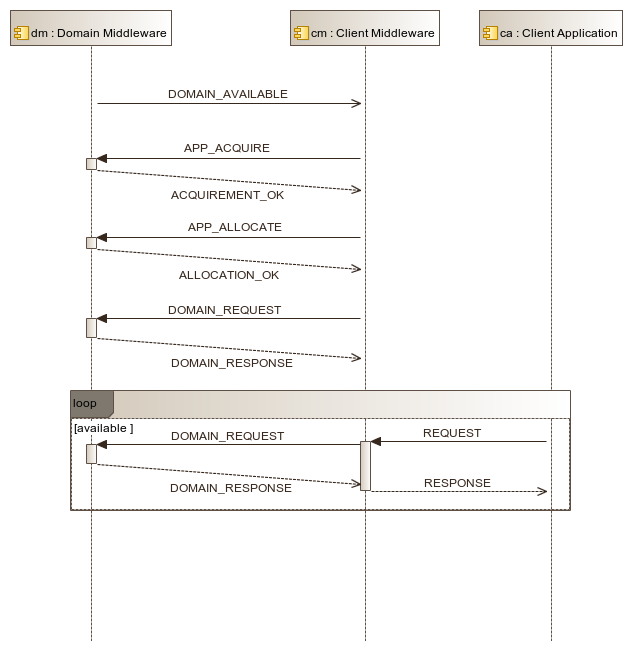
\includegraphics[width=0.6\textwidth]{figs/protocols.png}
  \caption{TODO}
  \label{fig:protocols}
\end{figure}
